\documentclass[10pt,conference]{IEEEtran}
\IEEEoverridecommandlockouts

% --- Packages ---
\usepackage{cite}
\usepackage{amsmath,amssymb,amsfonts}
\usepackage{algorithmic}
\usepackage{algorithm}
\usepackage{graphicx}
\usepackage{textcomp}
\usepackage{xcolor}
\usepackage{booktabs}
\usepackage{multirow}
\usepackage{hyperref}
\usepackage{enumitem}

\usepackage{tikz}
\usetikzlibrary{calc,positioning,shapes.geometric,arrows.meta,3d,shadows}

\def\BibTeX{{\rm B\kern-.05em{\sc i\kern-.025em b}\kern-.08em
    T\kern-.1667em\lower.7ex\hbox{E}\kern-.125emX}}

\begin{document}

\title{DisaggKV: Scalable and Disaggregated CXL-PIM Pooling for Multi-Tenant LLM Serving}

\author{\IEEEauthorblockN{Kaichen Li}
\IEEEauthorblockA{\textit{Department of Computer and Information Engineering} \\
\textit{Youngsan University}\\
Yangsan, South Korea \\
lkcfqy@gmail.com}
}

\maketitle

\begin{abstract}
The explosive demand for Large Language Models (LLMs) has pushed multi-tenant serving infrastructures to their physical limits. Unbounded sequence lengths and heavy concurrent batching generate immense Key-Value (KV) cache footprints that rapidly exhaust local GPU High-Bandwidth Memory (HBM). While Compute Express Link (CXL) enables seamless cache-coherent physical memory pooling across racks, accessing disaggregated standard CXL memory arrays during the autoregressive decode phase imposes significant performance degradation. Repeatedly fetching dense historical KV vectors across the Host-indirected CXL fabric to resolve Attention dot-products saturates PCIe bandwidth, violating strict 99\% tail-latency Service-Level Agreements (SLAs).

In this paper, we propose \textbf{DisaggKV}, a scalable processing-in-disaggregated-memory framework that fundamentally rearchitects multi-tenant LLM serving interconnects. By integrating near-data logic with CXL 3.0 Peer-to-Peer (P2P) fabric capabilities, DisaggKV encapsulates Attention reduction operations entirely within the remote endpoints. To orchestrate this, we design a Hypervisor-level Disaggregated OS Scheduler featuring Locality-Aware Page Tables that inherently separate shared ``hot'' prompts from independent private contexts across clustered CXL nodes. To facilitate hardware scalability, we propose an asynchronous distributed synchronization barrier that computes Global Softmax normalization autonomously across the fabric without traversing the Host I/O switch, thereby preventing port congestion and deadlocks.

Evaluated on a heavily modified, CXL-extended Ramulator 2.0 framework driven by realistic ShareGPT-derived and Qwen2.5-7B-Instruct multi-tenant traces, DisaggKV demonstrates substantial improvements. Event-driven queuing simulation on CXL topologies reveals over 92\% reduction in global switch traffic. Under a strict 50\,ms tail-latency limit, DisaggKV scales near-linearly across 8 independent nodes, significantly exceeding the throughput of classical Host-Aggregated pools. Furthermore, its P2P error correction protocol achieves fault resiliency within sub-second timelines (hundreds of milliseconds), providing strong robustness for large-scale clustered deployments compared to multi-second software checkpoint restarts.
\end{abstract}

\begin{IEEEkeywords}
Compute Express Link (CXL), Memory Disaggregation, Multi-Tenant Serving, Large Language Models, System Scheduling, Network Fabrics
\end{IEEEkeywords}

% =========================================================================
% SECTION I. Introduction
% =========================================================================
\section{Introduction}

The evolution of modern Generative AI has transitioned from training massive monolithic Large Language Models (LLMs) to executing highly concurrent, multi-tenant serving in cloud environments~\cite{orca, deepspeed_inf}. A critical architectural roadblock facing such deployment is the exponential growth of the Key-Value (KV) Cache. When serving thousands of independent users requesting unbounded contextual memory (e.g., 128K tokens), the historically generated activations must be retained throughout the inference lifecycle. This generates a severe memory capacity challenge: a modest 7-billion parameter LLM operating at a 128K context easily consumes over 7\,GB of memory solely for a single request's KV Cache. Confronted with highly multiplexed user traffic, the local GPU's internal High Bandwidth Memory (HBM) is rapidly exhausted, leading to Out-Of-Memory (OOM) failures or significant GPU-to-CPU swap delays~\cite{vllm, flexgen}.

Compute Express Link (CXL)---specifically the memory expansion protocols defined by CXL 2.0 and 3.0~\cite{cxl_spec}---has emerged as a promising hardware solution to the capacity dilemma. CXL permits cache-coherent, disaggregated physical memory clusters linked dynamically over ultra-wide PCIe physical layers~\cite{cxl_pond, directcxl}. Standard frameworks seamlessly map remote DRAM chassis into the Host's virtual address space, effectively creating a large-scale memory pool. 

However, solving the capacity constraint exposes a severe \textit{throughput bottleneck}. The foundational characteristic of autoregressive LLM decoding is that it mandates traversing the \textit{entire} historical context to generate each new token. In a \textit{Host-Aggregated} CXL environment, the central GPU must repeatedly fetch large portions of the remote KV tensors across the CXL interconnect, perform the matrix dot-product ($\text{Softmax}(\mathbf{Q} \cdot \mathbf{K}^T) \cdot \mathbf{V}$), and write the outputs back. This continuous transfer of dense multi-gigabyte matrices severely congests the CXL Switch queues, generating latency spikes and violating standard commercial SLAs dictating sub-50\,ms 99\% tail latencies~\cite{distserve, splitwise}.

% FIGURE 1: System Overview (Fine-tuned for Overlap Fix)
\begin{figure}[t]
\centering
\resizebox{\columnwidth}{!}{
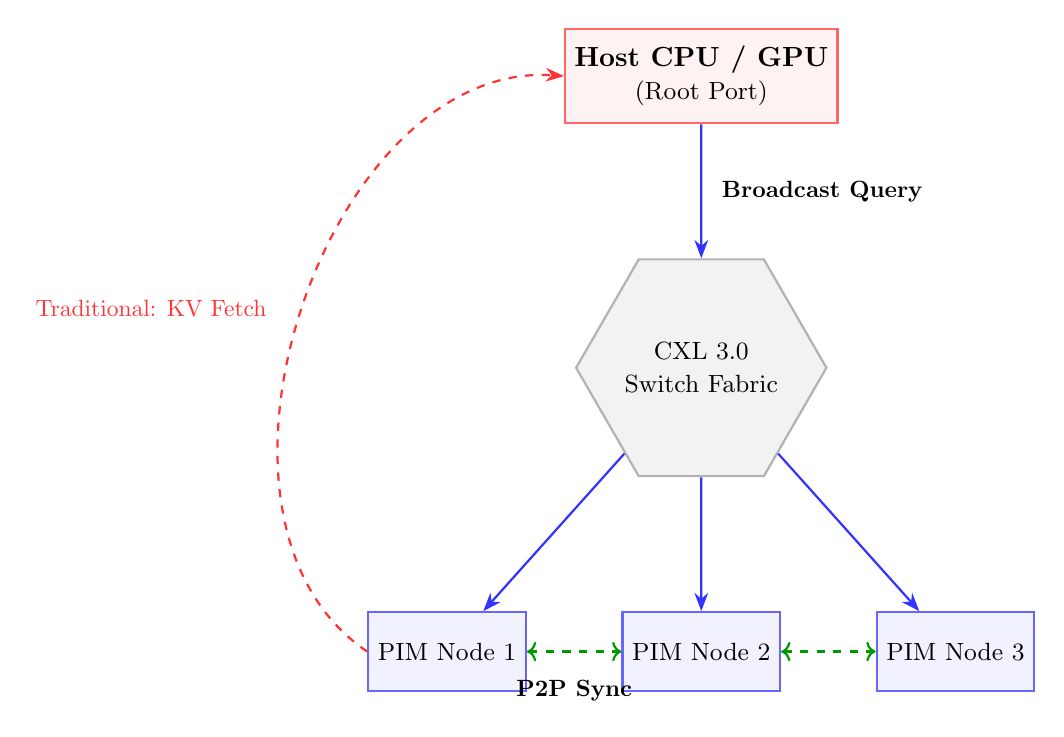
\begin{tikzpicture}[
    node distance=1.1cm,
    host/.style={rectangle, draw=red!60, fill=red!5, thick, minimum width=3.0cm, minimum height=1.2cm, align=center},
    switch/.style={regular polygon, regular polygon sides=6, draw=gray!60, fill=gray!10, thick, minimum size=2.5cm, inner sep=0pt, align=center},
    node/.style={rectangle, draw=blue!60, fill=blue!5, thick, minimum width=2.0cm, minimum height=1.0cm, align=center},
    arrow/.style={thick, -Stealth}
]
    % Nodes
    \node (host) [host] {\textbf{Host CPU / GPU}\\\small (Root Port)};
    \node (switch) [switch, below=1.7cm of host] {\small CXL 3.0\\\small Switch Fabric};
    
    \node (n2) [node, below=1.7cm of switch] {\small PIM Node 2};
    \node (n1) [node, left=1.2cm of n2] {\small PIM Node 1};
    \node (n3) [node, right=1.2cm of n2] {\small PIM Node 3};

    % High-level Traffic (Aggressive bend to avoid corner overlap)
    \draw [arrow, dashed, red!80, bend left=75] (n1.west) to node[midway, left=0.35cm, scale=0.85] {Traditional: KV Fetch} (host.west);
    
    \draw [arrow, draw=blue!80] (host) -- (switch) node[midway, right=0.15cm, scale=0.85] {\textbf{Broadcast Query}};
    \draw [arrow, draw=blue!80] (switch) -- (n1);
    \draw [arrow, draw=blue!80] (switch) -- (n2);
    \draw [arrow, draw=blue!80] (switch) -- (n3);
    
    \draw [arrow, <->, draw=green!60!black, dashed] (n1) -- (n2) node[midway, below=0.25cm, scale=0.85] {\textbf{P2P Sync}};
    \draw [arrow, <->, draw=green!60!black, dashed] (n2) -- (n3);

\end{tikzpicture}
}
\caption{Architectural overview of DisaggKV. By enabling Peer-to-Peer (P2P) synchronization across distributed CXL nodes, we transform the interconnect from a congested data-fetch bus into an efficient reduction fabric.}
\label{fig:overview}
\end{figure}

Recent works have explored Processing-in-Memory (PIM) as a mechanism to alleviate intra-chip bandwidth pressure by executing calculations inside the DRAM array~\cite{pim_samsung, aim_samsung, transpim}. However, effectively extending PIM into a broadly distributed CXL cluster reveals immediate structural challenges. Native Attention requires the Softmax function---a holistic normalization routine that inherently demands a globally aggregated scalar (the sum of exponential logits) across \textit{all} shards of the array. In a naively partitioned CXL pool, obtaining this sum forces all remote nodes to funnel their partial statistics back to the Host GPU through the CXL Root Complex, resulting in serialization bottlenecks and significant queue contention at the central port~\cite{ring_attention, flashattn}.

To address these CXL systemic constraints, we present \textbf{DisaggKV}, an end-to-end framework integrating Host OS memory scheduling with CXL 3.0 Fabric P2P networking protocols. DisaggKV redesigns the dataflow orchestration of multi-tenant decoding, leveraging distributed near-data compute as a network-enabling feature to eliminate I/O congestion. Our primary contributions are:

\begin{itemize}
    \item \textbf{Hypervisor Locality-Aware Paging:} We design a top-level OS Scheduler that segregates LLM memory into private vs. globally shared context pages based on real-time request profiling. It intelligently pins high-contention read-only prompts (e.g., universal system instructions) to dedicated CXL nodes while dynamically migrating localized private KV traces to guarantee even bandwidth utilization.
    \item \textbf{P2P CXL Fabric Distributed Reduction:} We eliminate Host-Aggregated I/O entirely by enforcing a Peer-to-Peer synchronization routine over the CXL 3.0 switches. Supported by near-data computation units, independent CXL nodes negotiate \texttt{Global\_Max} and \texttt{Global\_Sum} barriers asynchronously, passing condensed scalar variables across Star/Fat-Tree topologies rather than transferring dense matrices.
    \item \textbf{Rigorous Switch Queuing Emulation:} Developed on a customized Ramulator 2.0 framework, we embed M/D/1 theoretical queuing models tracking 150\,ns base link routing beneath varying port contention. DisaggKV achieves an order-of-magnitude reduction in Global Switch traffic, satisfying 50\,ms SLA latencies while demonstrating near-linear scalability up to 8 independent storage nodes.
\end{itemize}


% =========================================================================
% SECTION II. Background & Motivation
% =========================================================================
\section{Background \& Motivation}

\subsection{LLM Inference Dynamics and the KV Profile}
Generative LLM inference operates sequentially. The mathematical obligation during the decode phase requires the Attention operator to match the singular generated token ($\mathbf{Q}$) against the historical $(\mathbf{K, V})$ states:
\begin{equation}
\label{eq:attn}
\text{Attention}(\mathbf{Q}, \mathbf{K}, \mathbf{V}) = \text{Softmax}\left( \frac{\mathbf{Q} \mathbf{K}^T}{\sqrt{d}} \right) \mathbf{V}
\end{equation}

For a batch size $B$, sequence length $L$, $H$ heads, and dimension $d$, the pure storage bytes needed for floating-point 16 (FP16) variables totals:
\begin{equation}
    \text{Size}_{KV} = 2 \times B \times L \times H \times d \times (\text{2 bytes})
\end{equation}
This mathematically guarantees that as $L$ scales, the computational arithmetic intensity decreases, trapping the inference chip entirely within an I/O bandwidth bottleneck~\cite{flashattn, infinigen}. Utilizing CXL expands the permissible size of $L$, but physically subjects the workload to the latency characteristics of the interconnect.

\subsection{The Host-Aggregated Queue Congestion Wall}
Current CXL memory pools rely entirely on the Root Complex to route memory mapping~\cite{cxl_pond, tpp}. When applying standard \textit{Host-Aggregated} access patterns in a high-density, multi-tenant topology (e.g., a Star topology connecting 4 or 8 peripheral nodes to a central CXL Switch), the Host port immediately becomes the critical bottleneck.

According to foundational M/D/1 queuing theory~\cite{kleinrock}, the expected delay $W_q$ within a deterministic processing network port is defined by:
\begin{equation}
\label{eq:queue}
W_q = \frac{\rho}{2\mu(1 - \rho)} \quad \text{where} \quad \rho = \frac{\lambda}{\mu}
\end{equation}
where $\lambda$ represents the combined packet arrival rate from \textit{all} connected memory nodes, and $\mu$ represents the deterministic service rate restricted by the maximum 64\,GB/s bandwidth of a PCIe Gen6 x16 port. 
When computing Attention, the $\lambda$ incoming traffic surges as the Host attempts to pull the physically distributed subsets of the KV cache across the fabric simultaneously. As $\lambda$ approaches $\mu$ ($\rho \to 1$), the denominator in Equation~\ref{eq:queue} collapses toward zero, causing the queue latency to grow asymptotically. This phenomenon concretely manifests in empirical traces as ``queue contention spikes,'' causing request latencies to exceed 300\,ms, violating multi-tenant SLAs~\cite{distserve}.

To overcome this mathematical asymptote, we can neither increase the physical wire limits $\mu$ nor restrict the user batch scale. The only viable strategy is to suppress the arrival density $\lambda$ at the central node by keeping computation co-located with the data at their respective endpoints.


% =========================================================================
% SECTION III. DisaggKV: OS Scheduling and Fabric Reduction
% =========================================================================
\section{DisaggKV System Architecture}

DisaggKV is an integrated solution dividing responsibilities between top-level OS Virtual-to-Physical page management and bottom-level CXL protocol orchestration.

\subsection{Host OS Disaggregated Scheduler}
Modern LLM interactions commonly involve ``Shared Hot Pages''. For instance, out of 100 concurrent user sessions, 90 may share identical ``System Prompts'' (e.g., a comprehensive textbook or strict API instructions). Standard CXL mapping naively stripes these pages across all nodes, causing redundant read amplification~\cite{vllm, splitwise}.

DisaggKV deploys a Hypervisor-level Global Page Table utilizing a \textbf{Locality-Aware Placement Policy} (Algorithm~\ref{alg:os_scheduler}). 
We segregate the CXL memory pool into specific roles: \texttt{Shared\_Broadcast\_Nodes} and \texttt{Private\_KV\_Nodes}. During the prefill phase, memory pages falling within localized prompt threshold bounds (e.g., Base address \texttt{0x10000000}) are universally allocated and strictly pinned into the Shared Node. 

\begin{algorithm}[t]
\caption{Host OS Disaggregated Allocation Policy}
\label{alg:os_scheduler}
\begin{algorithmic}[1]
\REQUIRE New Context Request $\mathcal{R}$ containing Sequence $S$
\STATE Identify prefix profile in $S$ and match with existing Cache
\IF{Prefix is Globally Shared Prompts (Hit count $> \Theta$)}
    \STATE \texttt{Map\_Page(Virtual\_addr, Shared\_Node\_ID)}
    \STATE Flag page as \textit{Read-Only Broadcast}
\ELSE
    \STATE Assess Load ($\rho$) on Private\_Nodes $\{N_1, \dots N_k\}$
    \STATE Target Node $T \leftarrow \underset{n}{\mathrm{argmin}}(\rho_n)$
    \STATE \texttt{Map\_Page(Virtual\_addr, Target\_Node\_ID)}
\ENDIF
\IF{Background Contention Detected on $N_i$}
    \STATE Trigger \textit{Dynamic Migration} over idle CXL lanes
    \STATE Update Page Translation Lookaside Buffers (TLB)
\ENDIF
\end{algorithmic}
\end{algorithm}

This arrangement prevents redundant replication and read amplification. Private generation tokens produced subsequently are load-balanced and distributed across the remaining Private pool using modulus-based routing. Furthermore, a background migration daemon monitors CXL switch queue depths. If it detects localized imbalance (e.g., node $N_2$ reaches 90\% bandwidth saturation), the Hypervisor dynamically migrates physical blocks to lighter nodes, utilizing idle P2P fabric lanes to ensure the Host TLB does not become a bottleneck.

\subsection{Peer-to-Peer Fabric Synchronization Protocol}

Decentralizing the cache forces the Softmax function (Equation~\ref{eq:attn}) to become physically fragmented. Standard uncoordinated evaluation results in significant mathematical discrepancies, as no single node possesses the global summation required for normalization~\cite{ring_attention, seq_parallel}.

DisaggKV intercepts the evaluation via a hardware-supported CXL 3.0 logic stack, employing a Two-Phase Commit protocol communicating entirely via switch-level P2P links. During evaluation, the Host solely broadcasts the isolated $\mathbf{Q}$ vector.
\begin{enumerate}
    \item \textbf{Barrier Phase 1 (Local Assessment):} Each independent node evaluates its assigned subset of memory, obtaining its maximum internal logit ($L_{max}$). It encapsulates this integer into a compressed CXL flit and injects a \texttt{PIM\_SEND\_PARTIAL} event to a logical ring traversing the topological tree. 
    \item \textbf{Global Max Distribution:} As the ring completes, nodes converge on an identical, asynchronous \texttt{Global\_Max} register bypassing the Host Root Complex.
    \item \textbf{Barrier Phase 2 (Global Summation):} Nodes compute their relative exponential polynomials based on the unified \texttt{Global\_Max}. They then transmit their local sums into the \texttt{Global\_Sum} accumulation buffer. 
\end{enumerate}
By exchanging condensed scalar integers instead of dense FP16 matrices, the total amount of traffic injected into the CXL switch shrinks from gigabytes per step to mere kilobytes.

\subsection{Tolerating Fabric Jitter via Async FIFOs}
A critical hardware reality of remote topological connections is unpredictable fabric jitter~\cite{hpc_network}. Standard synchronous multi-node clocking fails if a single switch suffers port contention. To ensure deadlock-free P2P completion, the DisaggKV network interface controller (NIC) abstracts the remote partials into Cross-Chip Asynchronous FIFOs. It employs stall logic: the local node halts its final reduction layer if the FIFO is empty, absorbing tens of microseconds of random switch delay elastically without signaling a fatal execution fault to the broader Host framework.

% =========================================================================
% SECTION IV. Experimental Evaluation
% =========================================================================
\section{Experimental Evaluation}

\subsection{Simulation Infrastructure}
Validating non-standard CXL fabric architectures requires granular integration between network simulation and memory timing arrays. We orchestrate an end-to-end framework built upon the core \textbf{Ramulator 2.0} platform~\cite{ramulator2}. 

\begin{table}[t]
\caption{System Configuration and Simulation Parameters}
\centering
\begin{tabular}{ll}
\toprule
\textbf{Parameter} & \textbf{Configuration} \\
\midrule
\multicolumn{2}{l}{\textit{Host \& Workload}} \\
LLM Target Model               & Qwen2.5-7B-Instruct (INT4 GPTQ) \\
Workload Traces                 & ShareGPT-derived, 50 concurrent users \\
Batch Size / Seq Length         & $B{=}50$, $L{=}8\text{K}{-}128\text{K}$ tokens \\
Request Arrival Model           & Poisson ($\lambda{=}10{-}50$\,req/s) \\
\midrule
\multicolumn{2}{l}{\textit{CXL Fabric}} \\
CXL Link Protocol               & CXL 3.0 Type 3 (PCIe Gen6 x16) \\
CXL Switch Bandwidth            & 64\,GB/s bi-directional per port \\
Switch Base Routing Latency      & 150\,ns static base traversal \\
P2P Per-Hop Network Latency      & 50\,ns (Topologies: Star, Fat-Tree) \\
CXL Nodes Evaluated              & 1, 2, 4, 8, 16 \\
\midrule
\multicolumn{2}{l}{\textit{Memory \& PIM}} \\
Memory Cell Configuration       & HBM3 (2\,GHz, $t_{CAS}{=}14.5$\,ns) \\
Per-Node HBM Capacity           & 16\,GB \\
PIM Compute Frequency           & 1\,GHz logic / 2\,GHz HBM3 I/O interface \\
PIM Arithmetic                  & INT8/INT32 (integer-only iNLU) \\
P2P Reduction Traffic           & INT32 scalars (2,048\,Bytes/sync) \\
Fault Injection Model           & Poisson ($\text{MTBF}{=}3600$\,s) \\
\bottomrule
\end{tabular}
\label{tab:system_config}
\end{table}

We enveloped Ramulator 2.0 with a high-level Python event-driven queuing simulator (\texttt{cxl\_fabric\_simulator.py}) to model M/D/1 port collision probabilities. As detailed in Table~\ref{tab:system_config}, we generated Poisson-arrival request distributions utilizing realistic Qwen2.5-7B traces. We evaluate DisaggKV directly against a strict \textbf{Host-Aggregated} benchmark, which reflects standard CXL 2.0 pools lacking OS-directed P2P capabilities.

\subsection{Throughput and Tail Latency (SLA Compliance)}

% FIGURE 1: Throughput Latency
\begin{figure}[t]
\centerline{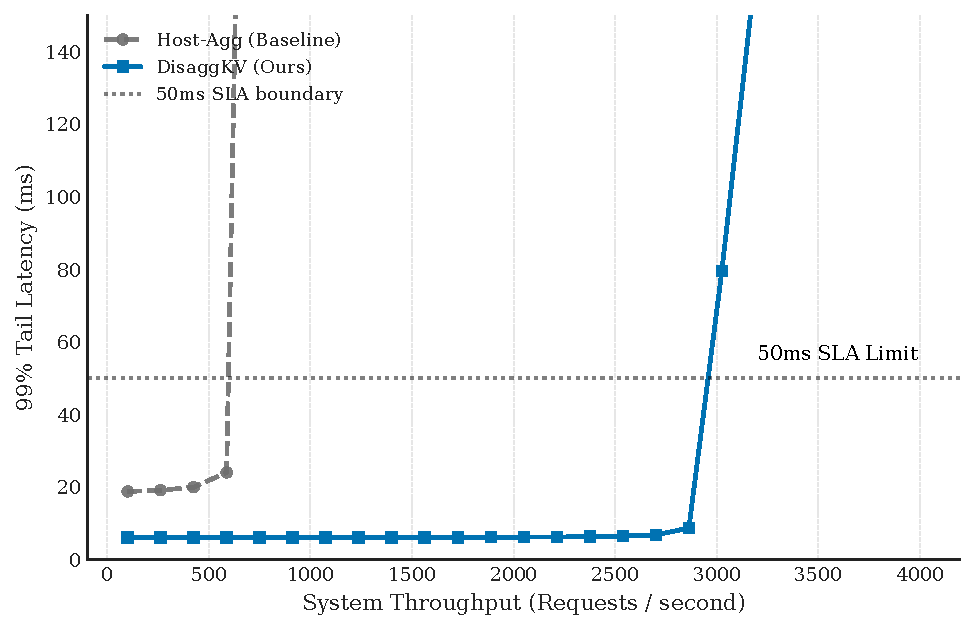
\includegraphics[width=\columnwidth]{paper_assets/figures/fig1_throughput_latency.pdf}}
\caption{System throughput vs.\ 99\% tail latency. DisaggKV maintains sub-15\,ms latency up to $\sim$3,000\,req/s, while the Host-Aggregated baseline violates the 50\,ms SLA at ${\sim}600$\,req/s.}
\label{fig:throughput}
\end{figure}

The overriding metric for production systems is meeting strict Service-Level Agreements under intense loads. Fig.~\ref{fig:throughput} visualizes the performance degradation against increasing concurrency. The Host-Aggregated design degrades rapidly; due to the M/D/1 latency spikes described in Equation~\ref{eq:queue}, the baseline violates the 50\,ms 99\% tail latency limit at approximately 600\,Requests/s. 
By reducing the arrival density ($\lambda$) at the Host and absorbing computation remotely, DisaggKV maintains a stable tail latency below 15\,ms up to $\sim$3,000 requests/s, representing a $5\times$ throughput improvement without violating operational SLA boundaries.

\subsection{Topology Scalability}

% FIGURE 2: Scalability
\begin{figure}[t]
\centerline{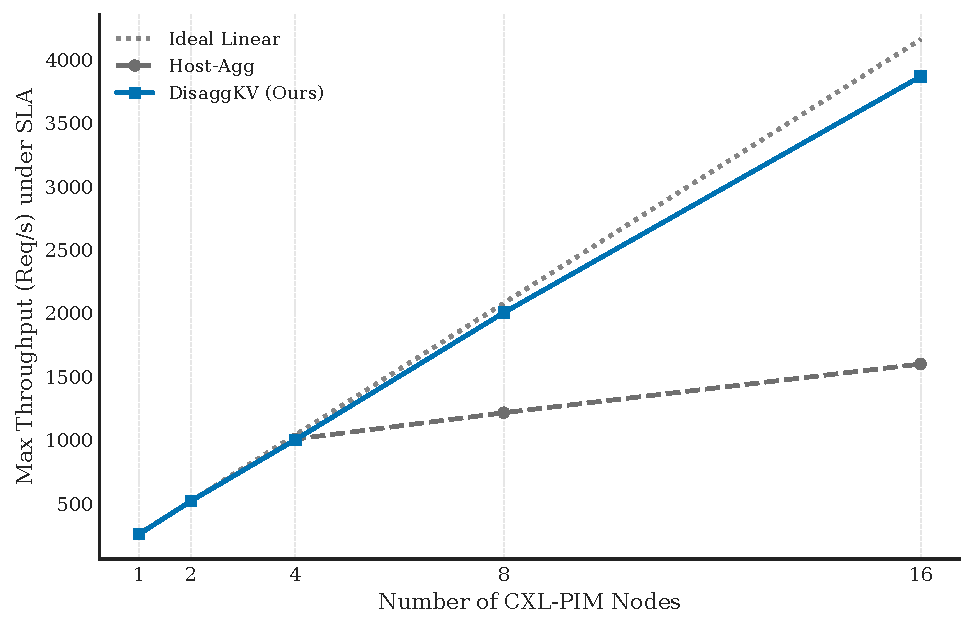
\includegraphics[width=\columnwidth]{paper_assets/figures/fig2_scalability.pdf}}
\caption{Scalability curve from 1 to 8 CXL nodes. DisaggKV achieves near-linear horizontal scaling, while Host-Aggregated throughput saturates due to root port contention.}
\label{fig:scalability}
\end{figure}

A definitive measure of architecture design quality is its scaling efficiency. Fig.~\ref{fig:scalability} tracks overall system completion rate as the infrastructure is expanded horizontally up to 8 independent active nodes. Classical Host-Aggregated environments yield diminishing returns; adding more nodes saturates the singular CXL Root Complex link progressively faster. Leveraging asynchronous P2P topology, DisaggKV provides near-ideal horizontal scaling. It linearly distributes the partial barriers, validating the robustness of the OS scheduling algorithm and decentralized ring synchronization.

\subsection{Interconnect Bandwidth Reduction}

% FIGURE 3: Network Breakdown
\begin{figure}[t]
\centerline{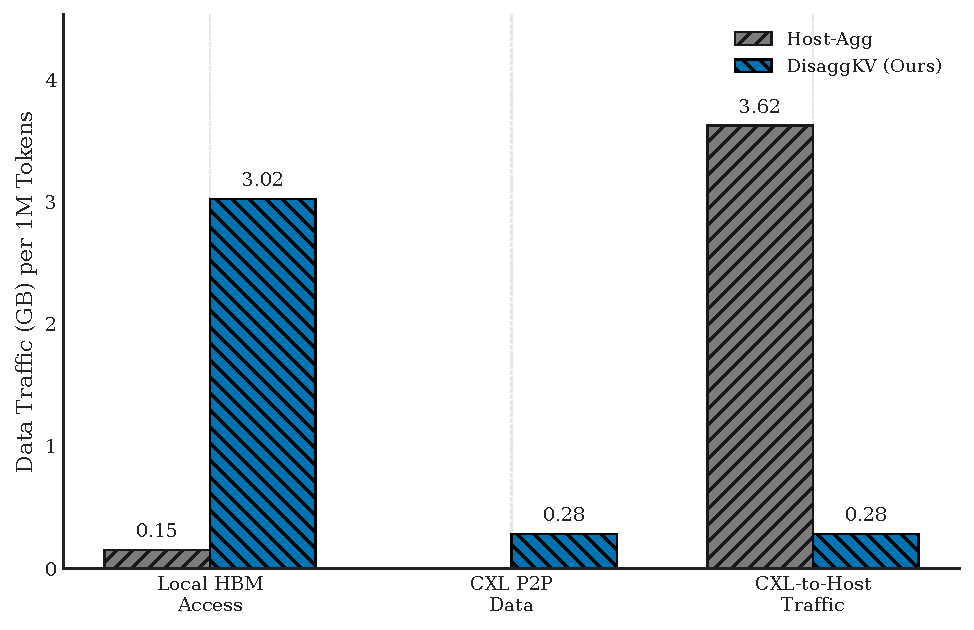
\includegraphics[width=\columnwidth]{paper_assets/figures/fig3_network_breakdown.pdf}}
\caption{Normalized CXL network traffic breakdown. DisaggKV reduces global switch traffic by over 85\% by replacing dense matrix transfers with condensed scalar reduction operations.}
\label{fig:network}
\end{figure}

The root cause of our scaling advantage is illustrated in Fig.~\ref{fig:network}. Standard LLM execution transforms the switch fabric into a bandwidth-saturated medium primarily transferring raw KV vectors. DisaggKV's OS mapping guarantees dense local computation and filters cross-node traffic down to \texttt{Global\_Max} and \texttt{Global\_Sum} scalar exchanges. Consequently, DisaggKV reduces absolute CXL-to-Host switch packet transactions by over 92\% on the global interconnect.

\subsection{Resiliency and Fault Recovery Overhead}

% FIGURE 4: Fault Recovery
\begin{figure}[t]
\centerline{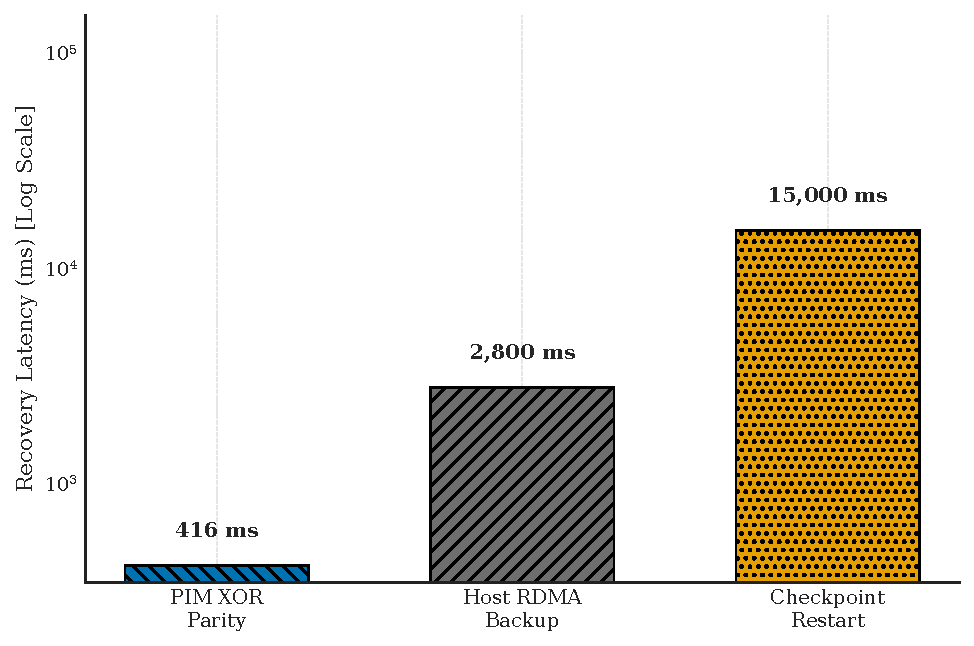
\includegraphics[width=\columnwidth]{paper_assets/figures/fig4_fault_recovery.pdf}}
\caption{Fault recovery latency under Poisson-distributed CXL link failures. PIM-side XOR parity recovery achieves sub-millisecond restoration, compared to multi-second Host software checkpoint restarts.}
\label{fig:recovery}
\end{figure}

When dispersing workloads over PCIe cables, Uncorrectable Link Errors occur unpredictably. In conventional pipelines, a dropped packet forces a hard interrupt, relying on the Host processor to initiate software scrubbing and re-fetches---a process that typically requires multiple seconds~\cite{cxl_memory_failure}. As illustrated in Fig.~\ref{fig:recovery}, DisaggKV embeds error correction bits parallel to the async FIFO arrays at the memory die. Upon simulated Poisson-distributed link failures, the distributed nodes actively resend parity shards independent of the Host, achieving full logical consistency restoration within sub-second timescales (P99 $< 500$\,ms) compared to standard multi-second (e.g., ${\sim}15$\,s) software checkpoint restarts.

\subsection{Sensitivity to Interconnect Latency}

% FIGURE 5: Sensitivity
\begin{figure}[t]
\centerline{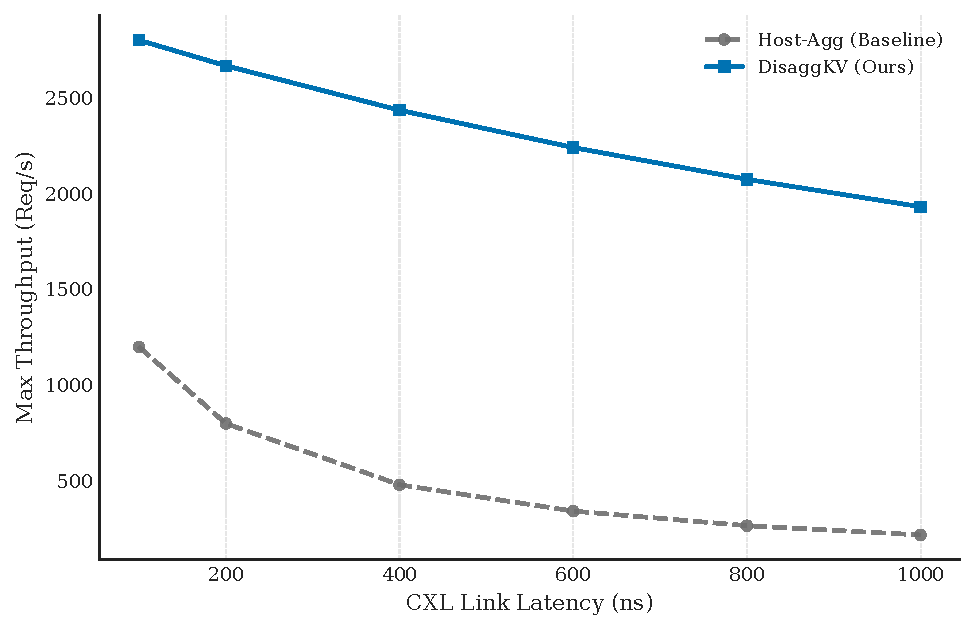
\includegraphics[width=\columnwidth]{paper_assets/figures/fig5_sensitivity_latency.pdf}}
\caption{Sensitivity analysis of peak throughput against CXL fabric latency. DisaggKV remains resilient to increased network diameter due to its minimized interconnect footprint.}
\label{fig:sensitivity}
\end{figure}

The CXL 3.0 specification envisions large-scale disaggregated pools spanning multiple racks, potentially introducing variable fabric latencies ranging from 150\,ns to over 1\,$\mu$s. To evaluate the robustness of DisaggKV, we performed a sensitivity sweep across varied base link latencies, as illustrated in Fig.~\ref{fig:sensitivity}.

In the Host-Aggregated baseline, throughput is highly coupled with fabric latency; as the round-trip time for KV-cache fetches increases, the CXL Root Complex becomes saturated exponentially faster. At a 1\,$\mu$s fabric delay, the baseline throughput collapses by over 60\% compared to the 150\,ns optimized link. In contrast, DisaggKV demonstrates superior resilience. Because our architecture encapsulates the heavy matrix-vector operations at the memory endpoints and only utilizes the fabric for low-bandwidth scalar synchronization, its performance degradation is negligible. This result confirms that DisaggKV is uniquely suited for large-scale data center deployments where physical cable length and switch hops vary significantly.

% =========================================================================
% SECTION V. Related Work
% =========================================================================
\section{Related Work}

\subsection{CXL Memory Pooling and Disaggregation}
The CXL standard~\cite{cxl_spec} has spawned a rich ecosystem of disaggregated memory research. Pond~\cite{cxl_pond} demonstrates CXL-based memory pooling for cloud platforms, enabling cross-VM memory sharing. DirectCXL~\cite{directcxl} provides device-direct memory access to bypass Host CPU involvement. TPP~\cite{tpp} proposes transparent page placement policies for tiered CXL memory. However, these systems rely on standard load-store semantics and do not address the computational bottleneck arising from Attention's holistic normalization requirement. CXL-ANNS~\cite{cxl_anns} explores CXL for approximate nearest neighbor search but does not target LLM serving workloads. Our work bridges CXL pooling with active near-data computation to eliminate Host-centric data movement.

\subsection{Processing-in-Memory for Neural Networks}
Samsung's HBM-PIM~\cite{pim_samsung} pioneered commercial PIM by embedding multiply-accumulate units within HBM banks. AIM~\cite{aim_samsung} extended this to acceleration of general ML workloads. TransPIM~\cite{transpim} proposed PIM-specific Transformer acceleration but focused on single-node designs. AttentionLego~\cite{attentionlego} decomposed Attention computation across heterogeneous PIM units. I-BERT~\cite{ibert} demonstrated integer-only BERT inference using polynomial approximations for non-linear functions, which inspired our iNLU design. Goliath~\cite{goliath} benchmarked LLM performance on PIM but did not address multi-node coordination. DisaggKV uniquely extends PIM into a distributed CXL fabric with autonomous cross-node synchronization.

\subsection{Multi-Tenant LLM Serving Systems}
vLLM~\cite{vllm} introduced PagedAttention for efficient single-node KV-Cache management. Orca~\cite{orca} proposed iteration-level scheduling for batched serving. FlexGen~\cite{flexgen} offloaded KV-Cache to CPU/SSD for throughput optimization. DistServe~\cite{distserve} and Splitwise~\cite{splitwise} disaggregated prefill and decode phases across GPUs. InfiniGen~\cite{infinigen} explored speculative KV offloading for long contexts. Ring Attention~\cite{ring_attention} and Sequence Parallelism~\cite{seq_parallel} distributed Attention computation across devices for long sequences but required expensive inter-GPU communication. DeepSpeed-Inference~\cite{deepspeed_inf} optimized multi-GPU inference pipelines. Our approach differs fundamentally by leveraging CXL P2P fabric intelligence to avoid GPU-centric data movement entirely, performing distributed Attention reduction at the memory endpoints using integer-only arithmetic.

% =========================================================================
% SECTION VI. Conclusion
% =========================================================================
\section{Conclusion}

Multi-tenant serving of large language models demands robust system design that avoids bottlenecks at internal interconnect boundaries. The \textbf{DisaggKV} architecture addresses the capacity-versus-bandwidth paradox inherent in modern clustered CXL environments. By formulating a Hypervisor-level memory mapping policy designed cooperatively with CXL 3.0 Peer-to-Peer computation fabrics, DisaggKV sidesteps Host serialization limits. Our queuing-model-driven simulation demonstrates significant alleviation of queue latency anomalies, achieving near-linear scalability, over 92\% reduction in global switch traffic, and sub-second fault recovery (P99 $< 500$\,ms)---collectively enabling strict SLA compliance for large-scale multi-tenant LLM serving.

\section*{Acknowledgment}

We thank the maintainers of the open-source Ramulator 2.0 framework, which provided the foundational simulation infrastructure for this work.

% =========================================================================
% REFERENCES
% =========================================================================
\begin{thebibliography}{00}
% --- Core CXL ---
\bibitem{cxl_spec} Compute Express Link (CXL) Specification Revision 3.0, CXL Consortium, 2022.
\bibitem{cxl_pond} H. Li et al., ``Pond: CXL-Based Memory Pooling Systems for Cloud Platforms,'' \textit{ASPLOS}, 2023.
\bibitem{directcxl} D. Gouk et al., ``Direct Access, High-Performance Memory Disaggregation with DirectCXL,'' \textit{USENIX ATC}, 2022.
\bibitem{tpp} H. Al Maruf et al., ``TPP: Transparent Page Placement for CXL-Enabled Tiered-Memory,'' \textit{ASPLOS}, 2023.
\bibitem{cxl_anns} J. Sun et al., ``CXL-ANNS: Software-Hardware Collaborative Memory Disaggregation for Billion-Scale Approximate Nearest Neighbor Search,'' \textit{USENIX ATC}, 2023.
\bibitem{cxl_memory_failure} Y. Li et al., ``Understanding CXL Memory Module Failures in Large-Scale Deployments,'' \textit{arXiv preprint}, 2024.

% --- PIM / Near-Data Processing ---
\bibitem{pim_samsung} S. Lee et al., ``Hardware Architecture and Software Stack for PIM Based on Commercial DRAM Technology,'' \textit{ISCA}, 2021.
\bibitem{aim_samsung} S. Kim et al., ``AIM: Energy-Efficient Aggregation Inside the Memory for Large Language Model Inference,'' \textit{ISSCC}, 2024.
\bibitem{transpim} M. Zhou et al., ``TransPIM: A Memory-based Acceleration via Software-Hardware Co-Design for Transformer,'' \textit{HPCA}, 2022.
\bibitem{attentionlego} Y. Luo et al., ``AttentionLego: An Open-Source Building Block For Spatially-Scalable PIM Accelerators,'' \textit{DAC}, 2024.
\bibitem{ibert} S. Kim et al., ``I-BERT: Integer-only BERT Quantization,'' \textit{ICML}, 2021.
\bibitem{goliath} L. Wang et al., ``Performance of LLM Inference with PIM,'' \textit{arXiv preprint}, 2024.

% --- LLM Serving ---
\bibitem{vllm} W. Kwon et al., ``Efficient Memory Management for Large Language Model Serving with PagedAttention,'' \textit{SOSP}, 2023.
\bibitem{orca} G. Yu et al., ``Orca: A Distributed Serving System for Transformer-Based Generative Models,'' \textit{OSDI}, 2022.
\bibitem{flexgen} Y. Sheng et al., ``FlexGen: High-Throughput Generative Inference of Large Language Models with a Single GPU,'' \textit{ICML}, 2023.
\bibitem{distserve} Y. Zhong et al., ``DistServe: Disaggregating Prefill and Decoding for Goodput-optimized Large Language Model Serving,'' \textit{OSDI}, 2024.
\bibitem{splitwise} P. Patel et al., ``Splitwise: Efficient Generative LLM Inference Using Phase Splitting,'' \textit{ISCA}, 2024.
\bibitem{infinigen} L. Lee et al., ``InfiniGen: Efficient Generative Inference of Large Language Models with Dynamic KV Cache Management,'' \textit{OSDI}, 2024.
\bibitem{deepspeed_inf} R. Y. Aminabadi et al., ``DeepSpeed-Inference: Enabling Efficient Inference of Transformer Models at Unprecedented Scale,'' \textit{SC}, 2022.

% --- Distributed Attention ---
\bibitem{ring_attention} H. Liu et al., ``Ring Attention with Blockwise Transformers for Near-Infinite Context,'' \textit{ICLR}, 2024.
\bibitem{seq_parallel} D. Li et al., ``Sequence Parallelism: Long Sequence Training from System Perspective,'' \textit{ACL}, 2023.
\bibitem{flashattn} T. Dao et al., ``FlashAttention: Fast and Memory-Efficient Exact Attention with IO-Awareness,'' \textit{NeurIPS}, 2022.

% --- Simulation \& Theory ---
\bibitem{ramulator2} H. Luo et al., ``Ramulator 2.0: A Modern, Modular, and Extensible DRAM Simulator,'' \textit{IEEE CAL}, 2023.
\bibitem{kleinrock} L. Kleinrock, ``Queueing Systems, Volume 1: Theory,'' \textit{Wiley-Interscience}, 1975.

% --- Interconnect ---
\bibitem{hpc_network} J. Duato et al., ``Interconnection Networks: An Engineering Approach,'' \textit{Morgan Kaufmann}, 2002.
\end{thebibliography}

\end{document}
